%  Robotics Text  by Jacob Rosen and Blake Hannaford
% (c) 2007  Jacob Rosen and Blake Hannaford
%

\chapter{Inverse Kinematics}



\section{Problem Statement and Learning Objectives}
% Problem Statement and Learning Objectives for Chapter 04
\paragraph{Problem Statement}
  
The inverse kinematics problem is to find the joint values for a given end effector configuration.  The solution to this problem is needed for most practical applications of serial robot arms. 

  
\paragraph{Learning Objectives}
Upon completing this Chapter, the reader should

\begin{itemize}
	\item Be able to plot the workspace of a serial manipulator with or without joint limits.
	\item Be able to solve for the joint angles of a planar robot given the end effector $x,y$ position and orientation.
	\item Be able to solve for the joint angles of a spatial 3 DOF robot given the $x,y,z$ position of the end effector.
	\item Be ready to tackle full scale inverse kinematics problems if sufficient time is available. 
\end{itemize}


\section{Overview}

We can express the forward kinematic problem as
\[
f(\theta) = {^0_6}T
\]
Then, to find the joint angles which correspond to a desired end effector configuration, we need to solve the inverse of this problem, the {\it Inverse Kinematic Problem}
\[
\theta = f^{-1}(^0_6T_d)
\]
where the $d$ subscript indicates the ``desired" end effector configuration.  Being able to solve the inverse kinematic problem is thus very important for automatic applications of robot manipulators since the control system must know the joint angles, $\theta$, in order to move the end effector to $^0_6T_d$.

For serial kinematic chains, this problem is harder than the forward kinematic problem.  Among the significant issues are:
\begin{itemize}
	\item Existence of solutions
	\item Multiple solutions
	\item How to find the solution(s)
\end{itemize}




\subsection{Workspace}
A robot arm, just like the human arm,  can only reach a certain number of points.  Wrapped up in our inverse kinematics calculation is the question of whether or not the desired end effector configuration is actually reachable.  Our mathematics should tell us this automatically when we try to compute the joint angles or displacements.  Fortunately, it works out that for a solution to the inverse kinematics problem to exist,  $^0_6T_d$ must be in the {\it workspace } of the manipulator.  We will use two definitions of workspace:

\begin{enumerate}
	\item {\bf Dexterous Workspace}.  The subset of space in which the robot end effector (EE) can reach all orientations.
	\item {\bf Reachable Workspace}   The subset of space in which the robot end effector (EE) can reach at least one orientation.
\end{enumerate}

Note that the dexterous workspace is a subset of the reachable workspace.

\begin{Example}
Consider a two link planar robot with no joint limits:

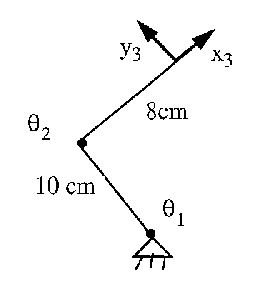
\includegraphics[width=1.5in]{figs04/00425.eps}

Then the reachable workspace is:


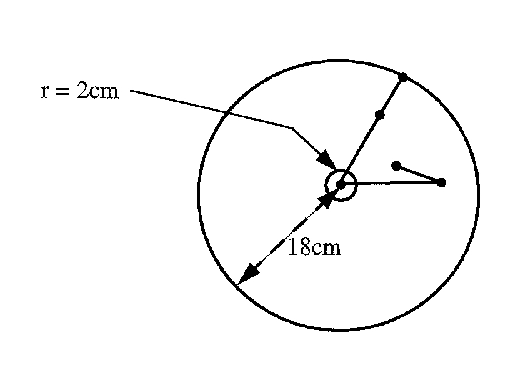
\includegraphics[width=3.125in]{figs04/00426.eps}

and the dexterous workspace is the empty set.

\newpage


Now, if $l_1 = l_2 = 9$, the outer radius is the same, and


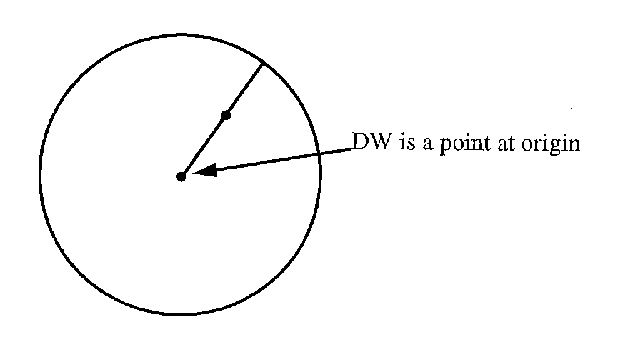
\includegraphics[width=3.75in]{figs04/00427.eps}

Now the RW is the same but the DW exists at a point at the origin where any orientation can be obtained.

\label{workspacedonut}
\end{Example}
\newpage
\begin{ExampleCont}

Now let's add a joint at the wrist

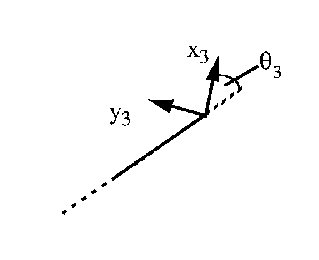
\includegraphics[width=1.5in]{figs04/00428.eps}


and set link lengths to $l_1 = 8,  = l_2 = 10 $.

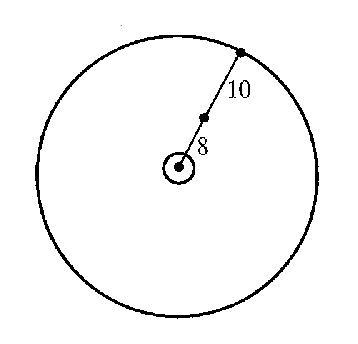
\includegraphics[width=2.0in]{figs04/00429.eps}

Now the reachable and dexterous workspaces are the same.
\end{ExampleCont}


\paragraph{Joint Limits}

The joints in real mechanisms often cannot achieve rotations of $0-2\pi$ (or for that matter infinite displacements on prismatic joints!).  Thus joint limits
\[
\theta_{imin} \le \theta_i \le \theta_{imax} \qquad d_{imin} \le d_i \le d_{imax}
\]
contribute additional limits to the workspace.

Rotary Joints

Without joint limits, the 2-link planar robot makes a donut shaped reachable workspace in the task space (Example \thechapter.\ref{workspacedonut}).  In joint space, any point can be attained.  When joint limits are introduced, a rectangular solid is created defined by $\theta_{imin}$ and $\theta_{imax}$ for each dimension.   To convert this rectangular solid back to task space, we note that each edge of the solid corresponds to varying just one joint at a time.  The edges in the joint space thus become arcs in the task space.   For the 2 joint manipulator, these limits allow joint configurations inside the rectangle shown in Figure \ref{2LinkVisJointLimits}, right.

\begin{figure}\centering
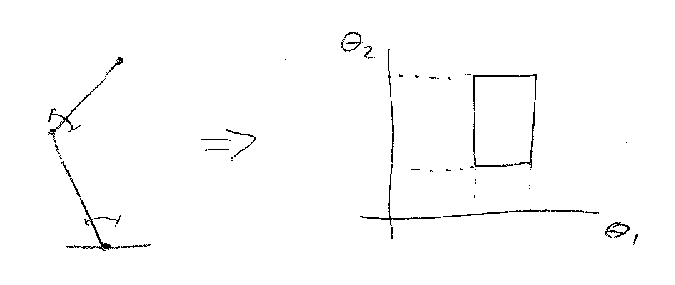
\includegraphics[width =4.0in]{figs04/00444.eps}
\caption{Visualization of joint limits for a 2-link manipulator.}\label{2LinkVisJointLimits}
\end{figure}



Plotting the workspace can be tricky with joint limits.   One approach:
\begin{enumerate}
	\item Identify the corners (vertices) of the joint space rectangular solid.
	\item Plot a point in the task space for each vertex.
	\item Connect the points with arcs (use a compass to draw) around the joint axis to connect the vertices.
	\item Remember that some workspace boundaries may not occur at joint limits such as when the arm is fully stretched out.
\end{enumerate}



%%%%%%%%%%%%%%%%%%%%%%%%%%%%%%%%%%%%%%%%%%%  4.2
\begin{ExampleSmall}\label{2LinkJointLimits}
Consider a 2DOF planar manipulator with link lengths $l_1 = 4, l_2 = 1.5$.    Assume the joints are limited to
\[
0 \le \theta_1 \le 180^{\circ}   \qquad   -90^{\circ} \le \theta_2 \le 180^{\circ}
\]

Plot the reachable workspace.

\includegraphics[width=4.25in]{figs04/00445.eps}

\end{ExampleSmall}

%%%%%%%%%%%%%%%%%%%%%%%%%%%%%%%%%%%%%%%%%%%  4.3
\begin{ExampleSmall}
Same problem as previous example:  $l_1 = 3, l_2 = 1.5$.    Assume the joints are limited to
\[
45^{\circ} \le \theta_1 \le 135^{\circ}   \qquad   -45^{\circ} \le \theta_2 \le 90^{\circ}
\]
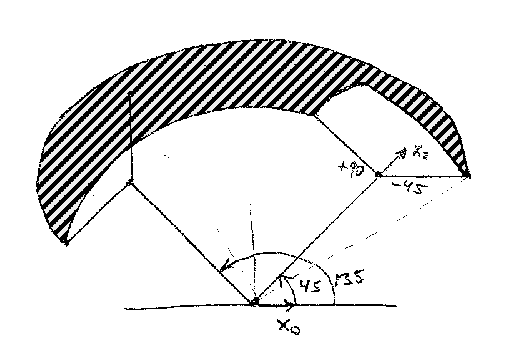
\includegraphics[width=4.25in]{figs04/00446.eps}
\end{ExampleSmall}


%%%%%%%%%%%%%%%%%%%%%%%%%%%%%%%%%%%%%%%%%%%   4.4
\begin{Example}
Generate top view and perspective view of the 3D workspace of the manipulator shown:

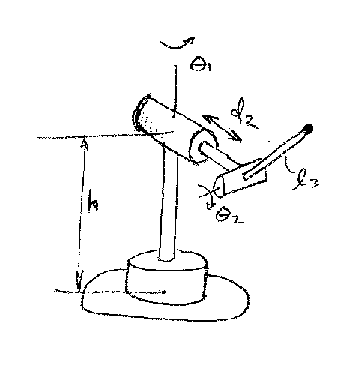
\includegraphics[width=2.5in]{figs04/00447.eps}

Where the joint limits are
\[
0 \le  \theta_1  \le 90^\circ     \qquad
2 <  d_2 < 4			 \qquad
-45^\circ  <  \theta_3 < 45^\circ
\]

First, we look at the plane containing the ``$d_2$" and the ``$l_3$" links (i.e. the vertical plane normal to $Z_2$.).

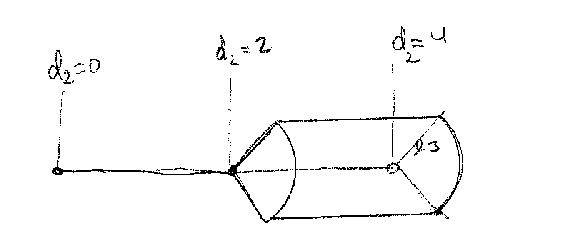
\includegraphics[width=4.25in]{figs04/00448a.eps}

Then by sweeping this planar workspace about $Z_1$, we generate the top view and perspective view.

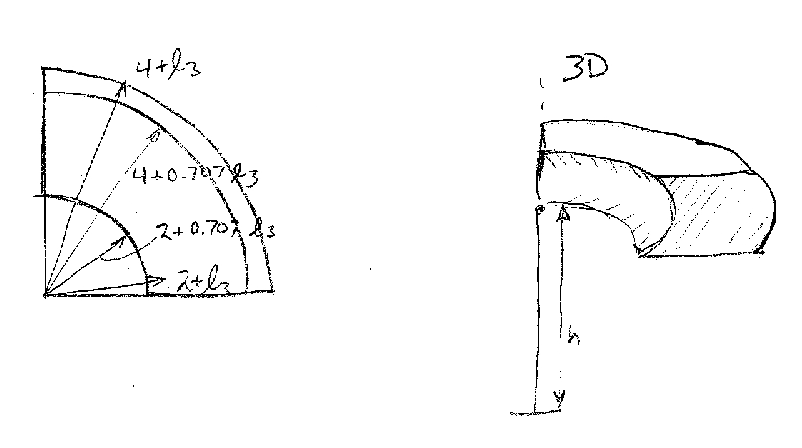
\includegraphics[width=4.25in]{figs04/00448b.eps}


\end{Example}


%%%%%%%%%%%%%%%%%%%%%%%%%%%%%%%%%%%%%%%%%%%%   4.5
\begin{Example}
Draw the 2-D workspace of the planar manipulator drawn below:

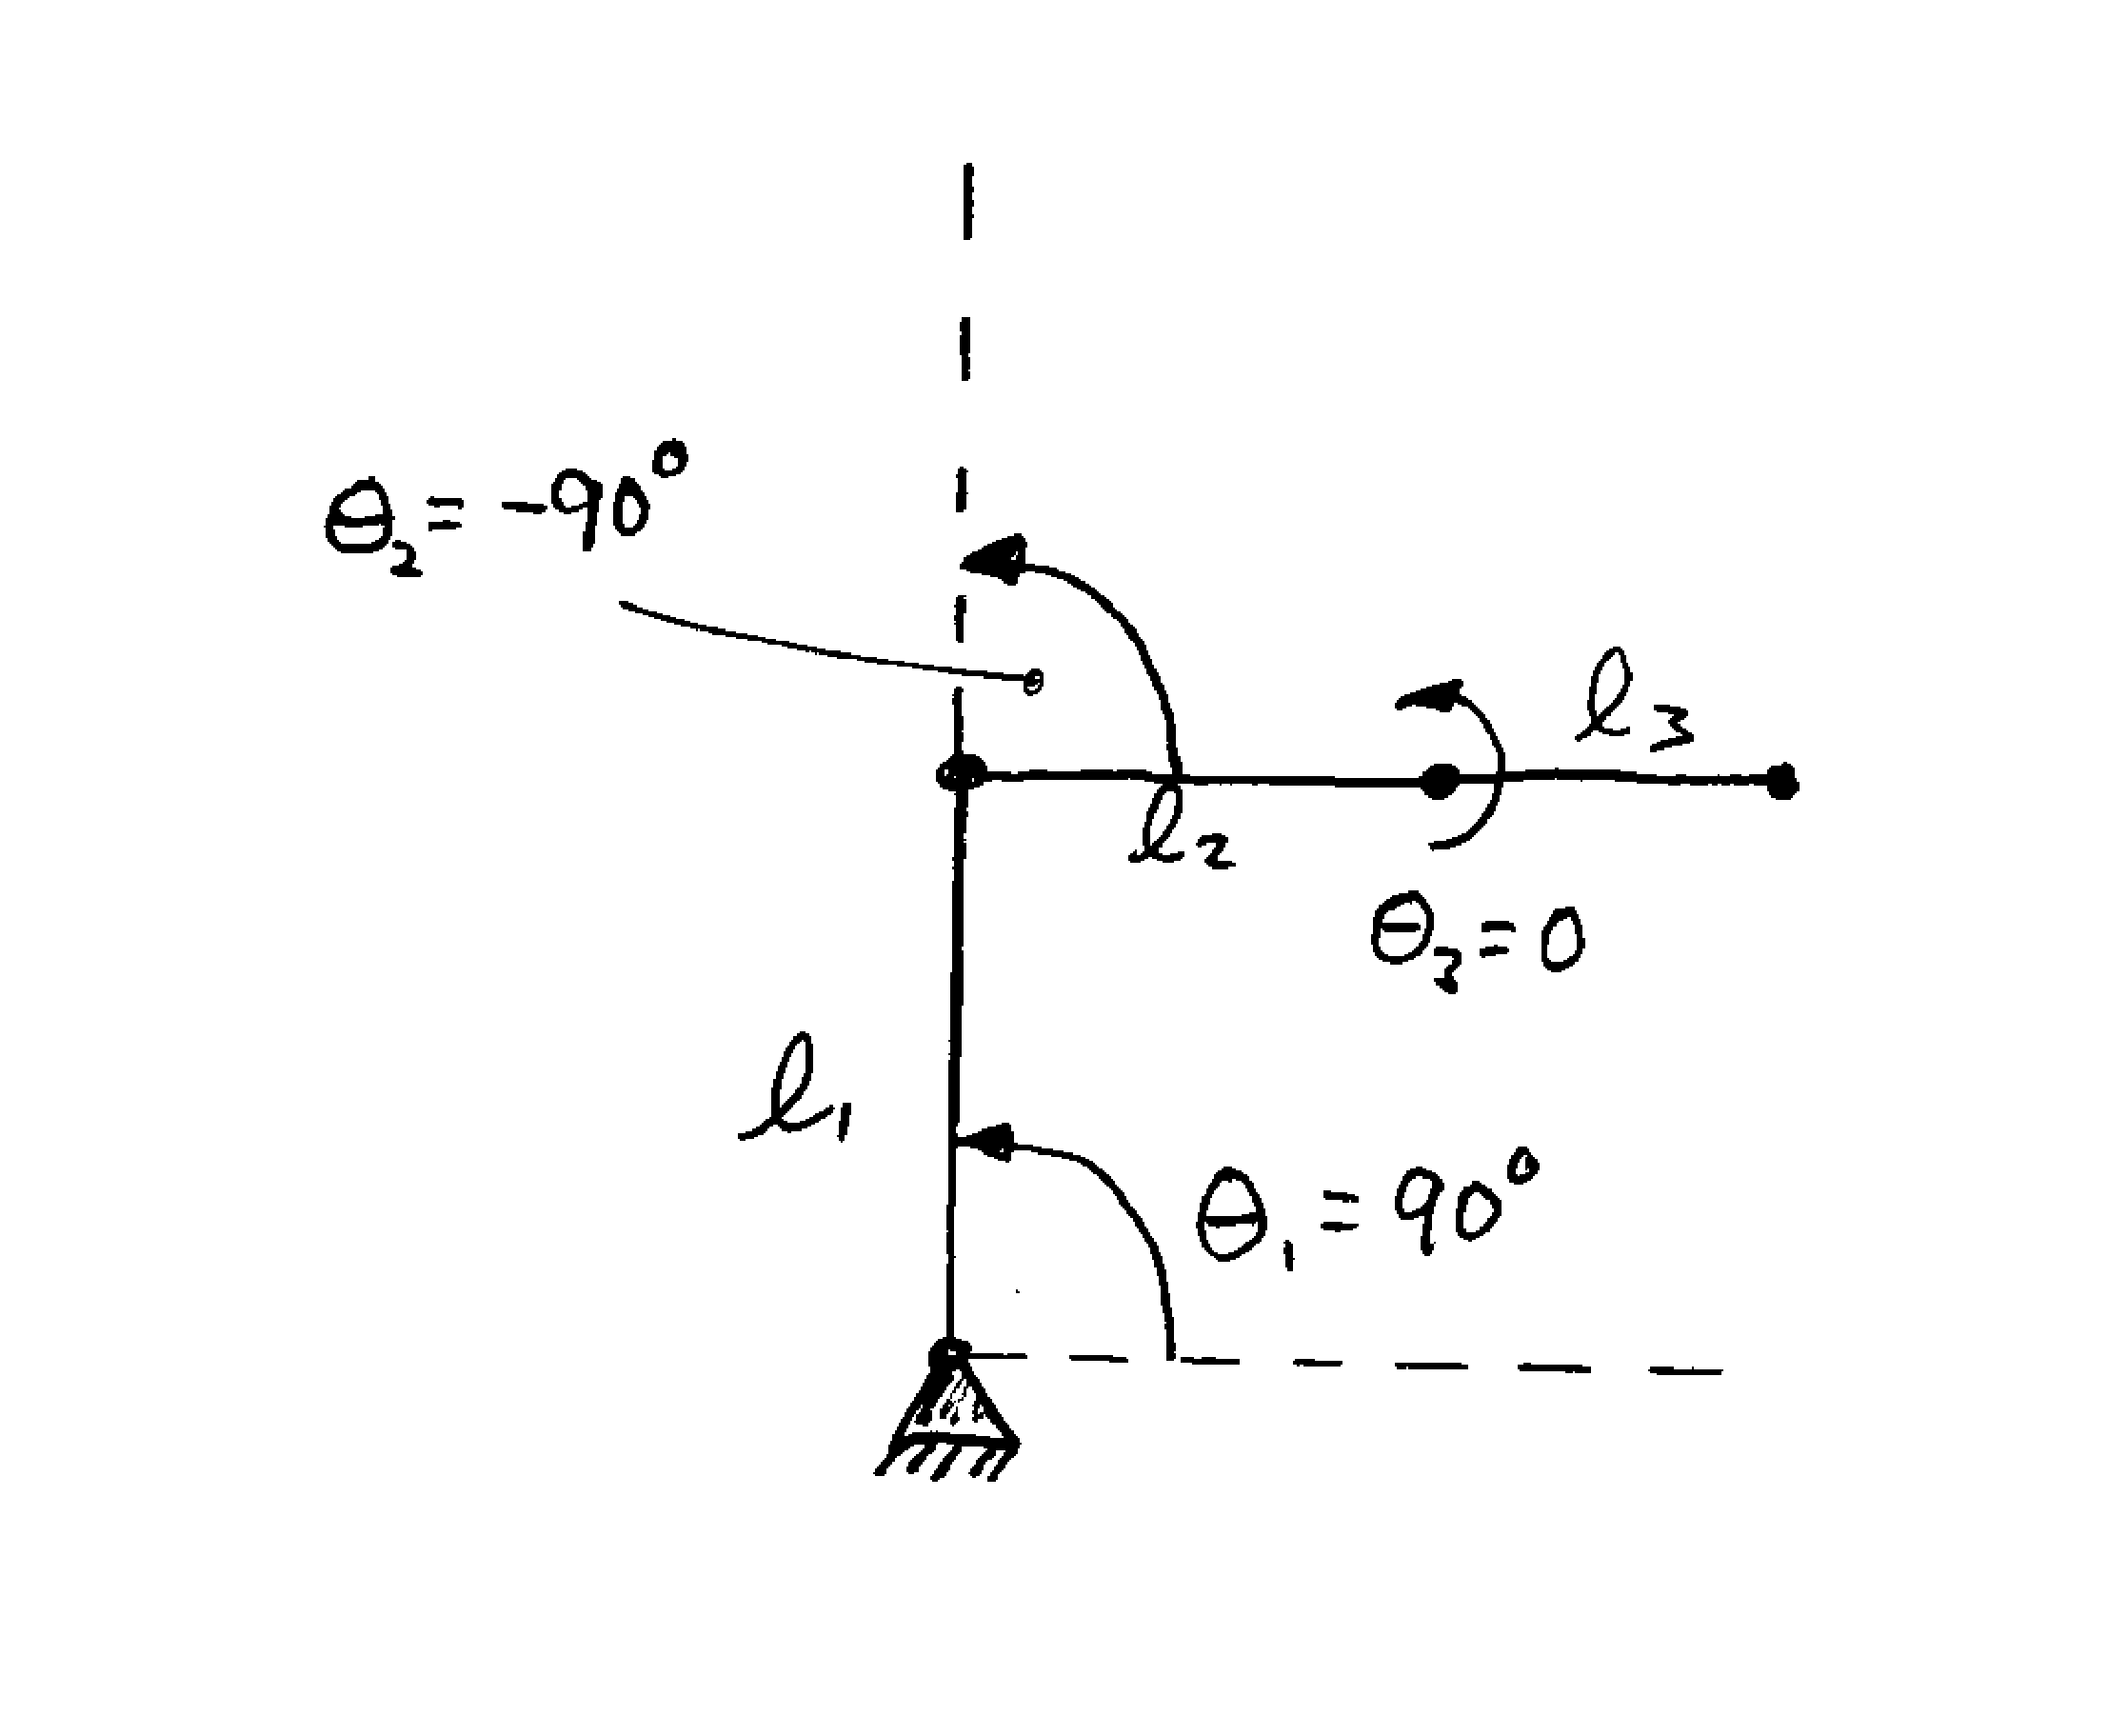
\includegraphics[width=3.0in]{figs04/00250.eps}

Facts:
\begin{itemize}
        \item $45^{\circ} < \theta_1   < 90^{\circ}$
        \item $-90^{\circ} < \theta_2  < 0^{\circ}$
        \item $20^{\circ} < \theta_3   < 120^{\circ}$
        \item $l_1 = 5, \quad l_2 = 4, \quad l_3 = 3$
\end{itemize}

\subsection*{Solution:}

\includegraphics[width=3.5in]{figs04/00442.eps}

\end{Example}












\subsection{Multiple Solutions}

We will consider two important cases: first, when the number of degrees of freedom of the robot are equal to the number in the task, and second when the number of degrees of freedom in the robot are greater than in the task.

1) Consider a 2 link planar arm (Figure \ref{2link3link}, left).

\begin{figure}\centering
\includegraphics[width=75mm]{figs04/00716.eps} \hspace{0.1in}
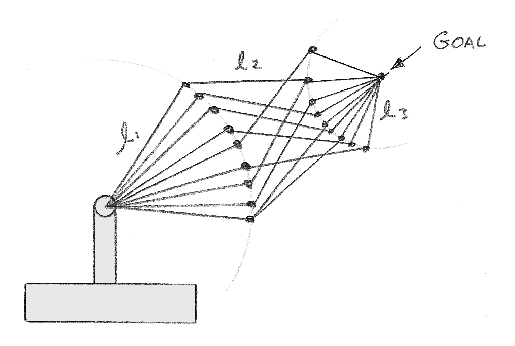
\includegraphics[width=75mm]{figs04/00717.eps}
\caption{Planar manipulators with 2 links (left) and 3 links (right) pointing at the same goal point.}\label{2link3link}
\end{figure}


This arm has two joints and two links.   We consider its task to be completely specified by the position of its end effector in the plane.  Thus the number of degrees of freedom and the dimensionality of the task are both 2.
In this case there are a finite number of solutions (2) which are illustrated above.   The planar two-joint arm can reach the goal in two configurations referred to as ``elbow-up" and ``elbow-down."  Each of these configurations is a separate solution to the inverse kinematics problem.

2) Consider a 3-link planar arm with the same goal(Figure \ref{2link3link}, right).



In this case there are an infinite number of solutions (10 are shown).  The robot has three joints and therefore three degrees of freedom, but the task is still only two DOF.   This robot is thus underspecified --- a situation we call kinematic redundancy.  A robot with kinematic redundancy
can even move itself around (among the infinite number of solutions) without moving the end effector from the goal.  This is called self-motion.
% Kinematic redundancy will be considered in Chapter \ref {KinematicRedundancyChapter}.




\subsection{Methods of Solution}

There are three principal ways to obtain the inverse kinematics solutions:

\begin{enumerate}
	\item ``Closed Form":  An analytic expression for $\theta$ as a function of $^0_6T_d$ which includes all solutions.

	\item Numerical methods.

	\item Hybrid approach in which some degrees of freedom are solved in closed form and others numerically.

\end{enumerate}

We will concentrate here on the closed form solution.


There are two standard approaches to obtaining the closed form solution, the algebraic approach, primarily involving manipulation of the forward kinematic equations, and the geometric approach, in which the inverse kinematics problem is reduced to one or more plane geometry problems. However, unlike the forward kinematics problem, there is no straightforward procedure which can be followed to get analytical solutions.

%*******************************************************************************************************************
%
%
\section{Inverse Kinematics Tools}
\subsection{Inverse of a Homogeneous Transform}
Let's define two frames which are related by a translation $P_{1,2}$ and a rotation $^1_2R$ (Figure \ref{positionrotationoffset}).

\begin{figure}\centering
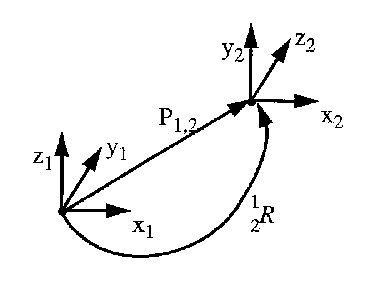
\includegraphics[width=2.5in]{figs04/00432.eps}
\caption{Two frames with a position offset, $P_{1,2}$ and a rotation offset ${^1_2R}$}\label{positionrotationoffset}
\end{figure}

If we represent this spatial relationship by a homogeneous transform, $T$, then it is reasonable to assume that an inverse, $T^{-1}$ must always exist

Q:  Why?

A:  One reason: a physical move can always be ``undone."   Another reason\footnote{J.M. McCarthy, ``Introduction to Theoretical Kinematics," MIT Press, 1990.},
eigenvalues of $T = 1, e^{j\theta}, e^{-j\theta}$, so their product, (the determinant) is always non-zero.

If the homogeneous transform is

\[
^1_2T =
\begin{bmatrix}
\begin{bmatrix}  &  &  \\  & ^1_2R&  \\ & & \\ \end{bmatrix}      &
 \begin{bmatrix}  \\ ^1P_{1,2} \\  \\ \end{bmatrix}            \\
 0 \quad 0 \quad 0      &   1
\end{bmatrix}
\]

then it is easy to show that its inverse is

\[
^1_2T^{-1} = ^2_1T =
\begin{bmatrix}
\begin{bmatrix}  &  &  \\  & ^2_1R&  \\ & & \\ \end{bmatrix}      &
 \begin{bmatrix}  \\ -^2P_{1,2} \\  \\ \end{bmatrix}            \\
 0 \quad 0 \quad 0      &   1
\end{bmatrix}
\]

where $^2_1R = {^1_2R}^T$ and $-^2P_{1,2} = {^2_1R}\left( -{^1P_{1,2}} \right )$


%%%%%%%%%%%%%%%%%%%%%%%%%%%%%%%%%%%%%%%%%%%%%%%%%%%%%%%%%%%%%%%%%%%%%%%%%%%%%%%%%%%%%%%%%%%%%%%%%%%%%%%%%%%%%%%%%%%
%%
%%    New quaternion material for inverse kinematics
%%
\subsection{Inverse of a Quaternion}

The inverse of a quaternion (Section \ref{QuaternionSection}), $q*$ ,is simply its conjugate, equation (\ref{quaternioninversedefinition}).

\[
q^* = \cos(\theta/2) - K_xi\sin(\theta/2) -K_yj\sin(\theta/2) - K_zk\sin(\theta/2) = (w,-x,-y,-z)
\]

\subsection{Inverse Sin and Cos}

The basic inverse trigonometric functions are often useful. Remember that they each have two solutions:
\[
\sin^{-1}(x) = \{\theta,\: \pi-\theta\} \qquad  \cos^{-1}(x) = \pm \theta
\]
and that they are only valid for
\[
-1 \leq x \leq 1
\]


\subsection{Atan2(y,x)}

We need a slightly more sophisticated form of the $\arctan()$ function to find angles.  Consider a trivial robot arm with a single link of unit length with a rotary joint at the origin.  If we pick a point on the unit circle, then the inverse kinematics problem is simply solved by the arctangent.  However, the arctan function domain is limited to the first and fourth quadrants:
\[
-\frac{\pi}{2} \leq \arctan(\frac{y}{x}) \leq \frac{\pi}{2}
\]

In real-world problems, we need to solve the inverse kinematics problem for any quadrant (Figure \ref{atan2figure}).

\begin{figure}\centering
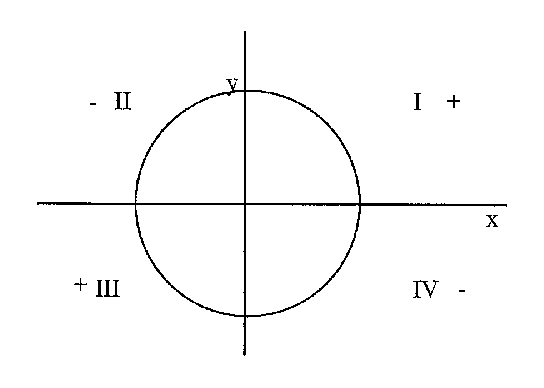
\includegraphics[width=3.25in]{figs04/00435.eps}
\caption{Unlike the arctangent function, the {\tt atan2(y,x)} function returns a result in any quadrant, I-IV.}\label{atan2figure}
\end{figure}


The {\bf atan2(y,x)} function, also known as the four quadrant arctangent, returns an angle between 0 and $2\pi$ allowing the solution to occupy any of the four quadrants.



\subsection{Key Trigonometric Identities}

Some trig identities (which may have faded from your mind) will be very useful in solving inverse kinematics problems.

\subsubsection{Sum of Angles}
If $c_{12} = \cos(\theta_1 + \theta_2)$ and $s_{12} = \sin(\theta_1 + \theta_2)$, then
\[
c_{12} = c_1 c_2 - s_1 s_2
\]
and
\[
s_{12} = c_1 s_2 + s_1 c_2
\]

This offers a way to solve   the following problem which frequently comes up in inverse kinematics:

\begin{quotation}
``Given $k_1$, $k_2$, and $x$, solve
$x = k_1\cos(\theta_1) + k_2\sin(\theta_1)$ for $\theta_1$.''
\end{quotation}

Here is one way:

Let $r = \sqrt{k_1^2 + k_2^2}$ and let $\theta_2 = \mathrm{atan2}(k_1,k_2)$.  In other words
\[
k_1 = rs_2, \quad k_2 = rc_2
\]
Rewriting the problem with this change of variables and applying sum-of-angles:
\[
x = rs_2c_1 + rc_2s_1 = rs_{12}
\]
\[
\frac{x}{r} = \sin(\theta_1 + \theta_2) = s_{12}
\]
We can solve this with the inverse sine function, $\sin^{-1}()$, but there is a preference in the robotics literature to transform it further into an atan2() solution by:
\[
c_{12} = \pm\sqrt{1-s^2_{12}} = \pm\sqrt{1-\left ( \frac{x}{r} \right)^2}
\]
\[
\theta_1 + \theta_2 = \mathrm{atan2}(s_{12}, c_{12})
\]
\[
\theta_1 = \mathrm{atan2}\left ( \frac{x}{r},  \pm\sqrt{1-\left ( \frac{x}{r} \right)^2} \right ) - \mathrm{atan2}(k_1,k_2)
\]

Note that there are two solutions to this equation corresponding to the $\pm$ choice of the square root.

A  joint angle can only be a real number for a reachable pose.  For the real solution to exist, the argument of the square root must be real giving
\[
\frac{x^2}{r^2}\leq 1, \quad x^2 \leq r^2, \quad |x| \leq |r|, \quad |x| \leq +\sqrt{k_1^2+k_2^2}
\]

So, if $|x| > \sqrt{k_1^2+k_2^2}$, no solution exists.  This is a mathematical test we can apply during computation to check whether or not the manipulator is capable of reaching the desired point.   However this is not the only condition which must be met in practice because we are still considering the idealized case where the joints can take on any value. In real manipulators, joint limits prohibit some points from being reached even if the inverse kinematics solution exists.


\subsection{Law of Cosines}

\begin{figure}\centering

\includegraphics[width=3.5in]{figs04/00436.eps}
\caption{Triangle and notation for the Law of Cosines.}\label{LOC}
\end{figure}

This old workhorse is a way to solve a frequently arising problem in inverse kinematics when an arm has two parallel axes.  Considering a triangle as in Figure \ref{LOC}, the law of cosines states:
\[
r^2 = L_1^2+L_2^2-2L_1L_2\cos(\theta)
\]
for an alternate form, we can use the fact that  $\theta = \pi + \alpha$ to get
\[
r^2 = L_1^2 + L_2^2 + 2L_1L_2\cos(\pm \alpha)
\]
This has two solutions since $\cos(\alpha) = \cos(-\alpha)$.


\subsection{Manipulator Sub-Space}

When the robot has fewer than six DOF, but the task has six DOF, then there are no solutions to the general problem, but only special cases. However, it is often useful to specify a subspace of the full 6 DOF configuration space which has a dimensionality which matches the robot arm.  For example, if we restrict our desired EE positions to the plane, then a planar arm is capable of reaching them. This plane, embedded in the six DOF space of possible rigid body configurations, in an example of a manipulator sub-space.

Alternatively, we can think of a planar world in which the configuration of any object consists of the $x$ and $y$ positions, and $\alpha$, the orientation of the object.

\begin{ExampleSmall}\label{PlanarManipSS}
Consider the following arm in a planar world which can reach various $x, y$ positions, but has a fixed wrist so that frame 3 has a particular orientation depending on the angles $\theta_1$ and $\theta_2$. Because of this dependence, the arm can only reach two specific orientations corresponding to the ``elbow-up" and ``elbow-down" solutions.

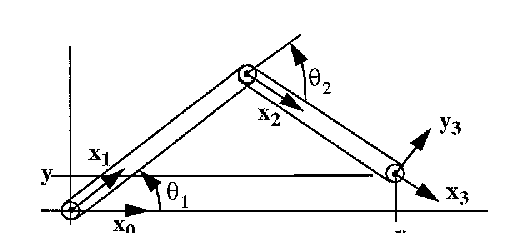
\includegraphics[width=3.75in]{figs04/00437.eps}


Suppose our task is described by
\[
^0_3T =
\begin{bmatrix}
\begin{bmatrix}  &  &  \\  & ^0_3R&  \\ & & \\ \end{bmatrix}      &
 \begin{bmatrix} x \\ y \\ z=0 \end{bmatrix}            \\
 0 \quad 0 \quad 0      &   1
\end{bmatrix}
\]

Since there is no joint at the wrist of this robot, ${^0_3R} = {^0_3R}(x,y)$ is a multivalued function of $x, y$.   We call

\[
^0_3T_D(x,y) =
\begin{bmatrix}
\begin{bmatrix}  &  &  \\  & ^0_3R(x,y) &   \\ & & \\ \end{bmatrix}      &
 \begin{bmatrix} x \\ y \\  0  \\ \end{bmatrix}            \\
 0 \quad 0 \quad 0      &   1
\end{bmatrix}
\]
the ``Manipulator subspace."  In more detail, we can only reach orientations in the $x,y$ plane so $^0_3R$ has the form
\[
{^0_3R}(x,y) =
   \begin{bmatrix}
          c\alpha	&   -s\alpha	&   0	\\
	  s\alpha	&    c\alpha	&   0	\\
	     0 		&     	0	&   1   \\
   \end{bmatrix}
\]
where $\alpha$ is a two-valued function of $x,y$.
If we use the algebraic approach, we would set up the problem:
\[
^0_3T_D(x,y) = {^0_1T}(\theta_1){^1_2T}(\theta_2){^2_3T}
\]
\end{ExampleSmall}

The manipulator sub-space is not always easy to find.  In the case of Example \thechapter.\ref{PlanarManipSS}, the inverse kinematics problem is more easily solved with a geometric approach and does not require a manipulator subspace anyway.  Sometimes 6 DOF robots are easier to solve than 5DOF robots because they do not require a manipulator subspace to be derived.





\subsection{Simultaneous Equations}

One problem which comes up frequently in inverse kinematics is simulataneous equations in the joint variables\footnote{Thanks to Dr. Pamela Bhatti.}.   For example,

\[
x = l_1c_1 + l_2c_{12}
\]
\[
y = l_1s_1 + l_2s_{12}
\]
where $c_{12} = \cos(\theta_1+\theta_2)$ (terms involving sums of two joint angles are common when two axes are parallel in a manipulator design).  The problem is to find $\theta_1$ when $\theta_2$ is known.

Use the sum-of-angles formulae to rewrite equations as

\[
x = l_1c_1 + l_2(c_1c_2 -s_1s_2)
\]
\[
y = l_1s_1 + l_2(c_2s_1 + s_2c_1)
\]

Now isolate the unknowns:

\[
x = (l_1+l_2c_2)c_1 - (l_2s_2)s_1
\]
\[
y = (l_1+l_2c_2)s_1 + (l_2s_2)c_1
\]


let $k_1 = (l_1+l_2c_2)$ and $k_2 = l_2s_2$ and place these equations into matrix form:

\[
\begin{bmatrix} x \\ y \end{bmatrix} =
\begin{bmatrix} k_1  & -k_2 \\ k_2 & k_1 \end{bmatrix}
\begin{bmatrix} c_1 \\ s_1   \end{bmatrix}
\]

Using standard $2\times2$ matrix methods to solve for $x,y$,

\[
\mathrm{determinant} = k_1^2 +k_2^2
\]
\[
c_1 = \frac {xk_1+yk_2}  {k_1^2 +k_2^2}
\]
\[
s_1 = \frac {yk_1-xk_2}  {k_1^2 +k_2^2}
\]

\[
\theta_1 = \mathrm{atan2}(yk_1-xk_2, \quad xk_1+yk_2)
\]
(Since the demoninators are always positive, we can drop them from the atan2. Also, note that
we need another equation to get $\theta_2$.)









\section{Algebraic Solution}

\subsection{Strategy}

The forward kinematics analysis of an all rotary  6DOF arm yields an equation
\[
^0_6T \quad = \quad ^0_1T(\theta_1) \quad ^1_2T(\theta_2) \quad ^2_3T(\theta_3) \quad ^3_4T(\theta_4) \quad ^4_5T(\theta_5) \quad ^5_6T(\theta_6)
\]
In the inverse kinematics version of the problem, ${^0_6T}$ is  known and we can call it ${^0_6T}_D$ (meaning desired), and the $\theta_i$ are unknowns.  The equation
\[
{^0_6T}_D = {^0_6T}
\]
is really 12 individual equations, one for each element of the first three rows.  On inspecting those 12 equations we might find one which can easily be solved for $\theta_1$ or perhaps a pair of equations which could jointly be solved for $\theta_1$.  But all of the other unknowns are mixed into complicated equations with no apparent solution.  However, when $\theta_1$ is solved,  $^0_1T(\theta_1)$ becomes a known matrix.  We can then write
% \[
%  ^0_1T(\theta_1)^{-1} \quad  ^0_6T \quad =  {^1_2T}(\theta_2) \quad {^2_3T}(\theta_3) \quad {^3_4T}(\theta_4) \quad {^4_5T}(\theta_5) \quad {^5_6T}(\theta_6)
% \]
\[
{^0_1T^{-1}}\;{^0_6T_D^{-1}} = {^0_1T(\theta_1)^{-1}}\;{^0_6T} \:
= \: {^1_2T}(\theta_2) \quad {^2_3T}(\theta_3) \quad {^3_4T}(\theta_4) \quad {^4_5T}(\theta_5) \quad {^5_6T}(\theta_6)
\]
which generates a fresh  set of 12 equations in which all the elements of the left hand side are knowns.    We may now find a new equation or set of equations which we can solve for $\theta_2$.   When $\theta_2$ is known, we can write
\[
 ^1_2T(\theta_2)^{-1} \quad {^0_1T}(\theta_1)^{-1} \quad {^0_6T}=   ^2_3T(\theta_3) \quad ^3_4T(\theta_4) \quad ^4_5T(\theta_5) \quad ^5_6T(\theta_6)
\]

Although there are several ``might"s in this description, because of the serial nature of the arms, this method works as described more often than one ``might" think.


\subsection{Examples}

\begin{Example}\label{ZYXWrist}
Consider a mechanism which corresponds to the $z,y,x$ Euler angles (Section \ref{ZYXEuler}).

\begin{center}
% 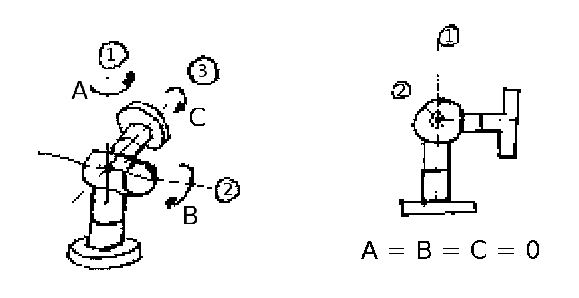
\includegraphics[width=3.6in]{figs04/00438.eps}
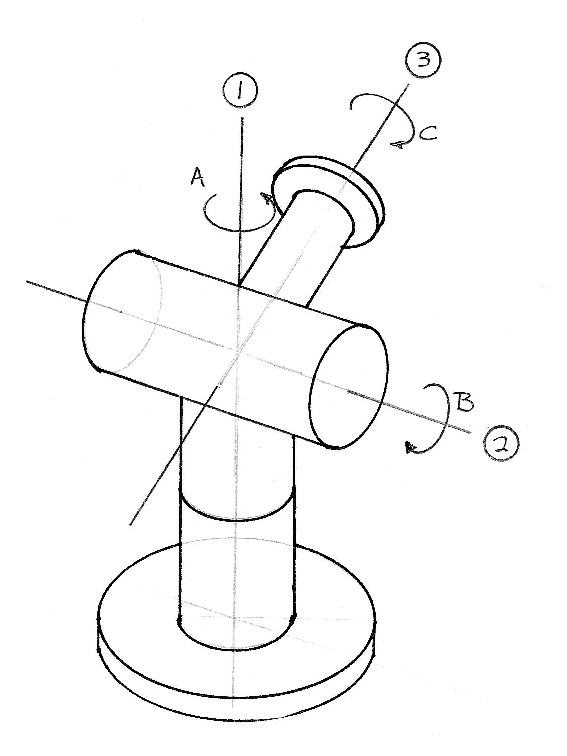
\includegraphics[width=2.2in]{figs04/00710.eps}
\includegraphics[width=1.943in]{figs04/00711.eps}
\end{center}

This mechanism has three axes of rotation which intersect at a single point.  The axes are arranged so that the first rotation about $z$, moves the $x$ and $y$ axes for subsequent rotations which corresponds to the definition of Euler angles.  The last frame, frame 3, has no offset from the point where the axes intersect, so the homogeneous transform consists only of rotation with no translation. The amounts of rotation about $z,y,x$ are $A,B,C$.   Expanding the 3x3 rotation matrix of Section \ref{ZYXEuler} into a 4x4 homogeneous transform with zero translation, we get
\[
{^0_3T}(A,B,C)  =
\begin{bmatrix}
cAcB  &  cAsBsC-sAcC    &  cAsBcC+sAsC  & 0  \\
sAcB  &  sAsBsC+cAcC    &  sAsBcC-cAsC  & 0  \\
-sB   &  cBsC           &    cBcC       & 0  \\
0     &     0           &      0        & 1  \\
\end{bmatrix}
\]
The manipulator subspace for this manipulator is
\[
^0_3T_D =
\begin{bmatrix}
\begin{bmatrix}  &  &  \\  &  R &   \\ & & \\ \end{bmatrix}      &
 \begin{bmatrix} 0 \\ 0 \\  0  \\ \end{bmatrix}            \\
 0 \quad 0 \quad 0      &   1
\end{bmatrix}
\]
Where $R$ can be any rotation matrix because we can reach nearly any orientation with ZYX Euler angles (see below).   The inverse kinematics problem can then be set up to solve
\[
^0_3T_D = {^0_3T}(A,B,C)
\]
for $A,B,C$, given $^0_3T_D$,     Expanding this equation gives
\[
\begin{bmatrix}
r_{11}    & r_{12}  & r_{13} \\
r_{21}    & r_{22}  & r_{23} \\
r_{31}    & r_{32}  & r_{33} \\
\end{bmatrix}
=\begin{bmatrix}
cAcB  &  cAsBsC-sAcC    &  cAsBcC+sAsC   \\
sAcB  &  sAsBsC+cAcC    &  sAsBcC-cAsC   \\
-sB   &  cBsC           &    cBcC
\end{bmatrix}
\]
Remember that everything on the left hand side is known as part of the desired EE configuration, and the unknowns are $A,B,C$.
\end{Example}

\begin{ExampleCont}
Looking over these 9 equations, we find fairly simple forms in the upper left hand corner:
\[
r_{11} = cAcB, \qquad r_{21} = sAcB
\]

We can add the squares of these equations together to get

\[
r_{11}^2 + r_{21}^2 = cB^2(cA^2 + sA^2)
\]
or
\[
cB = \pm\sqrt{r_{11}^2 + r_{21}^2}
\]
We can use more information from $^0_3T_D$ since $r_{31} = -sB$ and use atan2:
\[
B = \mathrm{atan2}(-r_{31},  \pm\sqrt{r_{11}^2 + r_{21}^2})
\]
if $B \ne \{ \pi/2, -\pi/2 \}$ then $cB$ is a non-zero constant and we can get
\[
A = \left \{ \begin{array}{cl}
                   \mathrm{atan2}( r_{21}, r_{11})      &   cB > 0         \\
                   \mathrm{atan2}(-r_{21},-r_{11})      &   cB \le 0
             \end{array}
    \right .
\]

Note that atan2(ay, ax) = atan2(y,x) if $a>0$ and that $\mathrm{atan2}(y,x) \ne \mathrm{atan2}(-y,-x)$.

Similarly


\[
r_{32} = cBsC, \qquad r_{33} = cBcC
\]
if $B \ne \{ \pi/2, -\pi/2 \}$ then $cB$ is a non-zero constant and we can get
\[
C = \left \{ \begin{array}{cl}
                   \mathrm{atan2}( r_{32}, r_{33})      &   cB > 0         \\
                   \mathrm{atan2}(-r_{32},-r_{33})      &   cB \le 0
             \end{array}
    \right .
\]
Alternatively we can express the multiple solutions slightly differently:

\[
C = \left \{ \begin{array}{cl}
                   \mathrm{atan2}( r_{32}, r_{33})      &   cB > 0         \\
                   \mathrm{atan2}(r_{32},r_{33}) + \pi      &   cB \le 0
             \end{array}
    \right .
\]

\end{ExampleCont}

\begin{Example}
Solve for $A,B,C$ in the wrist of Example \thechapter.\ref{ZYXWrist} where:
\[
{^0_3T}_D =
\begin{bmatrix}
0.925	&	0.018	&	0.379	\\
0.163	&	0.883	&	-0.441	\\
-0.342	&	0.470	&	0.814
\end{bmatrix}
\]

Solution:

\[
B = \mathrm{atan2} \left ( 0.342, \pm\sqrt{0.856+0.027} \right )
\]
\[
B = \{20^{\circ}, 160^{\circ}\}
\]

\[
A = \mathrm{atan2}(0.163, 0.925) = \arctan(0.176)  \quad (B = 20^{\circ})
\]
\[
A = \arctan(0.176)  + 180^{\circ}  \quad (B = 160^{\circ})
\]
\[
A = \{ 10^{\circ}, 190^{\circ} \}
\]


\[
C = \mathrm{atan2}(0.470, 0.814) = \arctan(0.577)  \quad (B = 20^{\circ})
\]
\[
C = \arctan(0.577)  + 180^{\circ}  \quad (B = 160^{\circ})
\]
\[
C = \{ 30^{\circ}, 210^{\circ} \}
\]

The solutions form a graph   which associates the multiple solutions of each
individual joint into two solution sets:
\[
[A_a, B_a, C_a], [A_b, B_b, C_b]
\]
\begin{center}
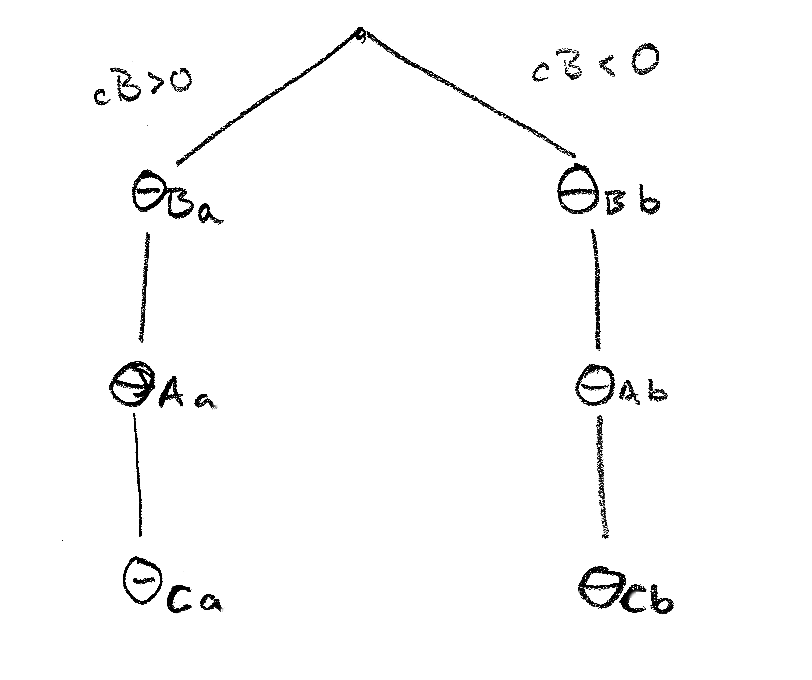
\includegraphics[width=2.5in]{figs04/sol_graph_wrist.png}
\end{center}

\end{Example}

\begin{Example}
{\bf Inverse Kinematics Example: ``Chair Helper'' 5-DOF Robot}

Problem and solution by Professor Melani Shoemaker.\\[0.25in]

\includegraphics[width=3.75in]{figs04/00441.eps}

Here is an example of solving the inverse kinematics equations for a 5-DOF robot embedded in 6-DOF space.
This is a robot designed to assist a wheelchair user.
By application of link frames, derivation of Denavit Hartenberg parameters, and applying them to the link
transform matrix,
\[
^{N-1}_NT = \left[
\begin{array}{cccc}
c\theta_N                 & -s\theta_N                    & 0               & a_{N-1} \\
s\theta_Nc\alpha_{N-1}    & c\theta_Nc\alpha_{N-1}        & -s\alpha_{N-1}  & -s\alpha_{N-1}d_N \\
s\theta_Ns\alpha_{N-1}    & c\theta_Ns\alpha_{N-1}        &  c\alpha_{N-1}  & c\alpha_{N-1}d_N  \\
0                         & 0                             &  0              & 1                 \\
\end{array}
\right]
\]
we can get the  transform for each link as follows:

\begin{tabular}{ll}
 &  \\
%
%  T01
%
$
^0_1T=\left[
\begin{array}{cccc}
1 & 0 & 0 & 0 \\
0 & 1 & 0 & 0 \\
0 & 0 & 1 & d \\
0 & 0 & 0 & 1
\end{array}
\right]
$
&
%
%   T12
%
$
^1_2T=\left[
\begin{array}{cccc}
c_2 & -s_2 & 0 & l_1 \\
s_2 & c_2 & 0 & 0 \\
0 & 0 & 1 & 0 \\
0  & 0 & 0 & 1
\end{array}
\right]
$

\\
 & \\
%
%   T23
%
$
^2_3T=\left[
\begin{array}{cccc}
c_3 &  -s_3 & 0 & 0 \\
0   &   0  & -1 & -l_2 \\
s_3 & c_3 & 0 & 0 \\
0  & 0 & 0 & 1
\end{array}
\right]
$
&
%
%   T34
%
$
^3_4T=\left[
\begin{array}{cccc}
c_4 &  -s_4 & 0 & 0 \\
0   &   0  & -1 & 0 \\
s_4 & c_4 & 0 & 0 \\
0  & 0 & 0 & 1
\end{array}
\right]
$
\\
 &  \\
%
%   T45
%
$
^4_5T=\left[
\begin{array}{cccc}
c_5 &  -s_5 & 0 & 0 \\
0   &   0  & 1 &  l_4 \\
-s_5 & -c_5 & 0 & 0 \\
0  & 0 & 0 & 1
\end{array}
\right]
$

& \\
& \\
\end{tabular}

Now we create the   forward kinematic equations,
by multiplying the link matrices together as:	%<hn>
\[
^0_5T= \quad ^0_1T \quad ^1_2T \quad ^2_3T \quad ^3_4T \quad ^4_5T
\]

\end{Example}
\begin{ExampleCont}
It turns out that if we start multiplying from $^4_5T$ and work our way backwards, we will get highly
useful intermediate results. i.e.
%Intermediate Results:
	%<*>
\[
^0_5T= \quad ^0_1T \quad ^1_2T \quad ^2_3T
\left[
\begin{array}{cccc}
 c_4c_5          & -c_4s_5             & -s_4           & -s_4l_4           \\
 s_5             & c_5                 & 0              & 0                 \\
 s_4c_5          & -s_4s_5             & c_4            & c_4l_4            \\
 0 & 0 & 0 & 1 \\
\end{array}
\right]
\]
The matrix at the right, $^3_5T$, will be useful later.    Similarly,	%<hn>
\[
^0_5T= \quad ^0_1T \quad ^1_2T
\left[
\begin{array}{cccc}
c_3c_4c_5-s_3s_5 & -c_3c_4s_5-s_3c_5 & -s_4c_3 & -c_3s_4l_4 \\
-s_4c_5 & s_4s_5 & -c_4 & -c_4l_4-l_2 \\
s_3c_4c_5+c_3s_5 & -s_3c_4s_5+c_3c_5 & -s_4s_3 & -s_3s_4l_4 \\
0 & 0 & 0 & 1
\end{array}
\right]
\]

	%<*hn>
This time the matrix at the right is $^2_5T$, and it will also be useful.
Continuing this process gives us the complete forward kinematic model:
\small{
\[
^0_5T =\left[
\begin{array}{cccc}
c_2c_3c_4c_5 - c_2s_3s_5 + s_2s_4c_5 & -c_2c_3c_4s_5-c_2s_3c_5-s_2s_4s_5 & -c_2s_4c_3+s_2c_4 & -c_2c_3s_4l_4+s_2c_4l_4+s_2l_2+l_1 \\
s_2c_3c_4c_5-s_2s_3s_5-c_2s_4c_5 & -s_2c_3c_4s_5-s_2s_3c_5+c_2s_4s_5 & -s_2s_4c_3-c_2c_4 & -s_2c_3s_4l_4-c_2c_4l_4-c_2l_2 \\
s_3c_4c_5+c_3s_5 & -s_3c_4s_5+c_3c_5 & -s_4s_3 & -s_3s_4l_4+d \\
0 & 0 & 0 & 1
\end{array} \right]
\]
}
%
%\small{
%\[
%^0_5T (\mathrm{cols} 1,2) =\left[
%\begin{array}{cc}
%c_2c_3c_4c_5 - c_2s_3s_5 + s_2s_4c_5 & -c_2c_3c_4s_5-c_2s_3c_5-s_2s_4s_5  \\
%s_2c_3c_4c_5-s_2s_3s_5-c_2s_4c_5 & -s_2c_3c_4s_5-s_2s_3c_5+c_2s_4s_5  \\
%s_3c_4c_5+c_3s_5 & -s_3c_4s_5+c_3c_5   \\
%0 & 0
%\end{array}\right]
%\]
%
%\[
%(\mathrm{cols} 3,4) =\left[
%\begin{array}{cc}
% -c_2s_4c_3+s_2c_4 & -c_2c_3s_4l_4+s_2c_4l_4+s_2l_2+l_1 \\
% -s_2s_4c_3-c_2c_4 & -s_2c_3s_4l_4-c_2c_4l_4-c_2l_2 \\
% -s_4s_3 & -s_3s_4l_4+d \\
% 0 & 1
%\end{array} \right]
%\]
%}
%
%\end{slide}
%\begin{slide}
%
	%<*>
We desire the robot to reach the configuration $^0_5T_D$, were
\[
^0_5T_D =
\left[
\begin{array}{cccc}
r_{11} & r_{12} & r_{13} & P_x \\
r_{21} & r_{22} & r_{23} & P_y \\
r_{31} & r_{32} & r_{33} & P_z \\
0&0&0&1\\
\end{array}
\right]
\]
%\end{slide}
%\begin{slide}
	%<*hn>
Remember, every element of $^0_5T_D$ is {\it known}.   We generate equations to solve by equating like
terms between $^0_5T_D$ and the forward kinematic model.   For example, to pick a small one,
%Each pair of elements is equation:
	%<*>
\[
r_{33} = -s_4s_3
\]

	%<*hn>
So far so good, but how do we attack this mess?
Unfortunately, there is no substitute for just going to a quiet room, getting a
cup of coffee, and going at it.   Here is what Melani did.
Let's look in particular at two equations we can write from the above:
%Start with two:
	%<*>
\[
r_{13} = -c_2s_4c_3+s_2c_4
\]
and
\[
P_x = -c_2c_3s_4l_4+s_2c_4l_4+s_2l_2+l_1
\]
If we 	%<hn>
re-write the second one as	%<*>
\[
P_x = (-c_2s_4c_3+s_2c_4)l_4+s_2l_2+l_1
\]
%\end{slide}
%\begin{slide}
	%<*hn>
we now have the right-hand-side of $r_{13}$ embedded inside the RHS of
$P_x$.   Therefore we can
substitute to get rid of the unknowns $ s_2, c_2, s_4, c_4$.	%<*>
\[
P_x = r_{13}l_4 + s_2l_2 + l_1
\]
This can be solved (because {\it only} $s_2$ is unknown) to give	%<hn>
\[
s_2 = \frac{P_x-r_{13}l_4 -l_1}{l_2}
\]
We can use the exact same logic on the second row of the matrix to get	%<hn>
\[
c_2 = \frac{-P_y-r_{23}l_4}{l_2}
\]
Now we have the first result:

\[
\theta_2 = \mathrm{atan2}(P_x-r_{13}l_4 -l_1,-P_y-r_{23}l_4)
\]
(note that we could take out the $\frac{1}{l_2}$ term because it is common to both	%<hn>
arguments of atan2 and because it is positive.)	%<hn>

\end{ExampleCont}
\begin{ExampleCont}
What else can we solve?   Let's use this same trick on the third row.	%<hn>
%Third row, same trick:
\[
r_{33} = -s_4s_3
\]
\[
P_z = -s_3s_4l_4 + d
\]
This   gives our second result:	%<hn>
\[
d = P_z - r_{33}l_4
\]
Now it seems like we have run out of  such tricks, but this is where our intermediate results	%<hn>
come to the rescue. We had	%<hn>
%Recall intermediate results:
\[
^0_5T= \quad ^0_1T \quad ^1_2T
\left[
\begin{array}{cccc}
c_3c_4c_5-s_3s_5 & -c_3c_4s_5-s_3c_5 & -s_4c_3 & -c_3s_4l_4 \\
-s_4c_5 & s_4s_5 & -c_4 & -c_4l_4-l_2 \\
s_3c_4c_5+c_3s_5 & -s_3c_4s_5+c_3c_5 & -s_4s_3 & -s_3s_4l_4 \\
0 & 0 & 0 & 1
\end{array}
\right]
\]
Since we know $d$ and $\theta_2$, $^0_1T$ and $ ^1_2T$ are now known.  Thus we	%<hn>
can write	%<hn>
\[
(^1_2T)^{-1}   (^0_1T)^{-1} \quad  {^0_5T} =
\left[
\begin{array}{cccc}
c_3c_4c_5-s_3s_5 & -c_3c_4s_5-s_3c_5 & -s_4c_3 & -c_3s_4l_4 \\
-s_4c_5 & s_4s_5 & -c_4 & -c_4l_4-l_2 \\
s_3c_4c_5+c_3s_5 & -s_3c_4s_5+c_3c_5 & -s_4s_3 & -s_3s_4l_4 \\
0 & 0 & 0 & 1
\end{array}
\right]
\]
%\end{slide}
%\begin{slide}
Let's define:
\[
\hat{T} = (^1_2T)^{-1}   (^0_1T)^{-1}  \quad {^0_5T_D}
\]
	%<*hn>
Though we
can't know the values of $\hat{T}$ until $d$ and $\theta_2$ are solved,  after that
point  we can use $\hat{T}$ the same way we used $^0_5T_D$. In other words, we can treat $\hat{T}$ as {\it known}.
\[
\hat{T} = \quad ^2_5T
\]
%
%We can write:
%\begin{center}
%\small{(known)} $\hat{T} = \quad ^2_5T$ \small{(unknown)}
%\end{center}
	%<*>
Equating elements we get
\[
\hat{T}_{33} = -s_4s_3
\]
\[
\hat{T}_{13} = -s_4c_3
\]
If $s_4 \neq 0$, we can treat it like a constant, but since both $\theta_3$ and	%<hn>
$\theta_4$ are unknown, we get two possible solutions:	%<hn>
%Two possible solutions
\[
\theta_{3,1} = \mathrm{atan2}(\hat{T}_{33},\hat{T}_{13} )
\]
and	%<hn>
\[
\theta_{3,2} = \mathrm{atan2}(-\hat{T}_{33},-\hat{T}_{13}) = \theta_{3,1}+ \pi
\]
Now that we have two solutions for $\theta_3$, we have $^2_3T_1$ and  $^2_3T_2$.	%<hn>
We can   generate two versions of a third {\it known} matrix:	%<hn>
%using both solutions of $\theta_3$:
\[
\tilde{T1} = (^2_3T_1)^{-1} (^1_2T)^{-1}   (^0_1T)^{-1}  \quad {^0_5T_D}
\]
\[
\tilde{T2} = (^2_3T_2)^{-1} (^1_2T)^{-1}   (^0_1T)^{-1}  \quad {^0_5T_D}
\]
These can be equated to our first intermediate result from the forward	%<hn>
kinematics to easily get $\theta_4$ and $\theta_5$:	%<hn>
%using first intermediate result: $^3_5T$
\[
\tilde{T}_{13} = -s_4, \quad \tilde{T}_{33}= c_4
\]
\[
\tilde{T}_{21} = -s_5, \quad \tilde{T}_{22}= c_5
\]

\end{ExampleCont}
\begin{ExampleCont}

but remembering that there are two versions of $\tilde{T}$
\[
\theta_{4,1} = \mathrm{atan2}(-\tilde{T1}_{13}, \tilde{T1}_{33})
\]
\[
\theta_{4,2} = \mathrm{atan2}(-\tilde{T2}_{13}, \tilde{T2}_{33})
\]
\[
\theta_{5,1} =\mathrm{atan2}(-\tilde{T1}_{21}, \tilde{T1}_{22})
\]
\[
\theta_{5,2} =\mathrm{atan2}(-\tilde{T2}_{21}, \tilde{T2}_{22})
\]


\subsection*{Recap}
	%<*hn>
To summarize, the result of our analysis is a general solution to the
inverse kinematics problem {\it for this robot} that will work for any reachable end
effector configuration, $^0_5T_D$.  Suppose we were now to implement this as a
piece of computer code, what would we have to do?  Here is a rough outline:
	%<*>
\begin{enumerate}
\item Read in the desired end-effector configuration
\[
^0_5T_D =
\left[
\begin{array}{cccc}
r_{11} & r_{12} & r_{13} & P_x \\
r_{21} & r_{22} & r_{23} & P_y \\
r_{31} & r_{32} & r_{33} & P_z \\
0&0&0&1\\
\end{array}
\right]
\]

\item Check that this matrix represents a valid
reachable pose for this robot
(see below).	%<hn>

\item
\[
\theta_2 = \mathrm{atan2}(P_x-r_{13}l_4 -l_1,-P_y-r_{23}l_4)
\]

\item
\[
d = P_z + r_{33}l_4
\]

\item Using the values of $\theta_2$ and $d$ just computed, compute
\[
\hat{T} = (^1_2T)^{-1}   (^0_1T)^{-1}  \quad {^0_5T_D}
\]

	%<*hn>
\item Verify assumption that $\theta_4 \neq 0$ or $\pi$. To do this,
we could
check that $|\hat{T}_{33}|$ {\bf and} $|\hat{T}_{13}|$ are greater than
zero, or we could check $|\hat{T}_{23}| < 1$.
If these tests fail, we can only solve for $\theta_3 + \theta_5$.
%
%\item Verify $\theta_4 \neq 0$ or $\pi$:
%\[
%|\hat{T}_{23}| < 1
%\]
	%<*>
\item
Compute
\[
\theta_{3,1} = \mathrm{atan2}(\hat{T}_{33},\hat{T}_{13} )
\]
\[
\theta_{3,2} = \theta_{3,1}+ 3.1415926
\]

\item
Using the values of $\theta_2$, $\theta_3$, and $d$ just computed, compute
\[
\tilde{T1} = (^2_3T_1)^{-1} (^1_2T)^{-1}   (^0_1T)^{-1}  \quad {^0_5T_D}
\]
\[
\tilde{T2} = (^2_3T_2)^{-1} (^1_2T)^{-1}   (^0_1T)^{-1}  \quad {^0_5T_D}
\]


\item Finally we can compute the joint angles:
\[
\theta_{4,1} = \mathrm{atan2}(-\tilde{T1}_{13}, \tilde{T1}_{33})
\]
\[
\theta_{4,2} = \mathrm{atan2}(-\tilde{T2}_{13}, \tilde{T2}_{33})
\]
\[
\theta_{5,1} =\mathrm{atan2}(-\tilde{T1}_{21}, \tilde{T1}_{22})
\]
\[
\theta_{5,2} =\mathrm{atan2}(-\tilde{T2}_{21}, \tilde{T2}_{22})
\]
\end{enumerate}

\end{ExampleCont}
\begin{ExampleCont}


\subsection*{Reachability}

We have skipped one last detail which makes the problem a bit more tricky.   The solution above
will only work if $^0_5T_D$ represents a valid reachable configuration for our manipulator.
Since we have only 5 degrees of freedom, not all orientations are possible at a given position.
It is not trivial to generate the $^0_5T_D$ matrix but we will leave that topic to another time.

\end{ExampleCont}








\section{Geometric Solution}

The other major approach to inverse kinematics is to identify and solve for joint angles or displacements by means of plane geometry.  Although the manipulator moves through 3D space, often a plane can be identified which always contains one or more mechanism joints and which contains a solvable triangle.  Before we see this type of situation, let us assume that we are dealing with manipulators that are confined to the plane.

\subsection{Planar Examples}
\begin{ExampleSmall}

\includegraphics[width=3.5in]{figs04/00087.eps}


First, assume that joint 3 is locked.
For $\theta_3 = 90^\circ$, find $\theta_1,$ and $d_2$, given the end effector
coordinates $x,y$:
\[
^0P_4 = \left[
\begin{array}{c}
x\\
y\\
\end{array}
\right]
\]
How many solutions are there and how do you find them?

\subsection*{Solution:}

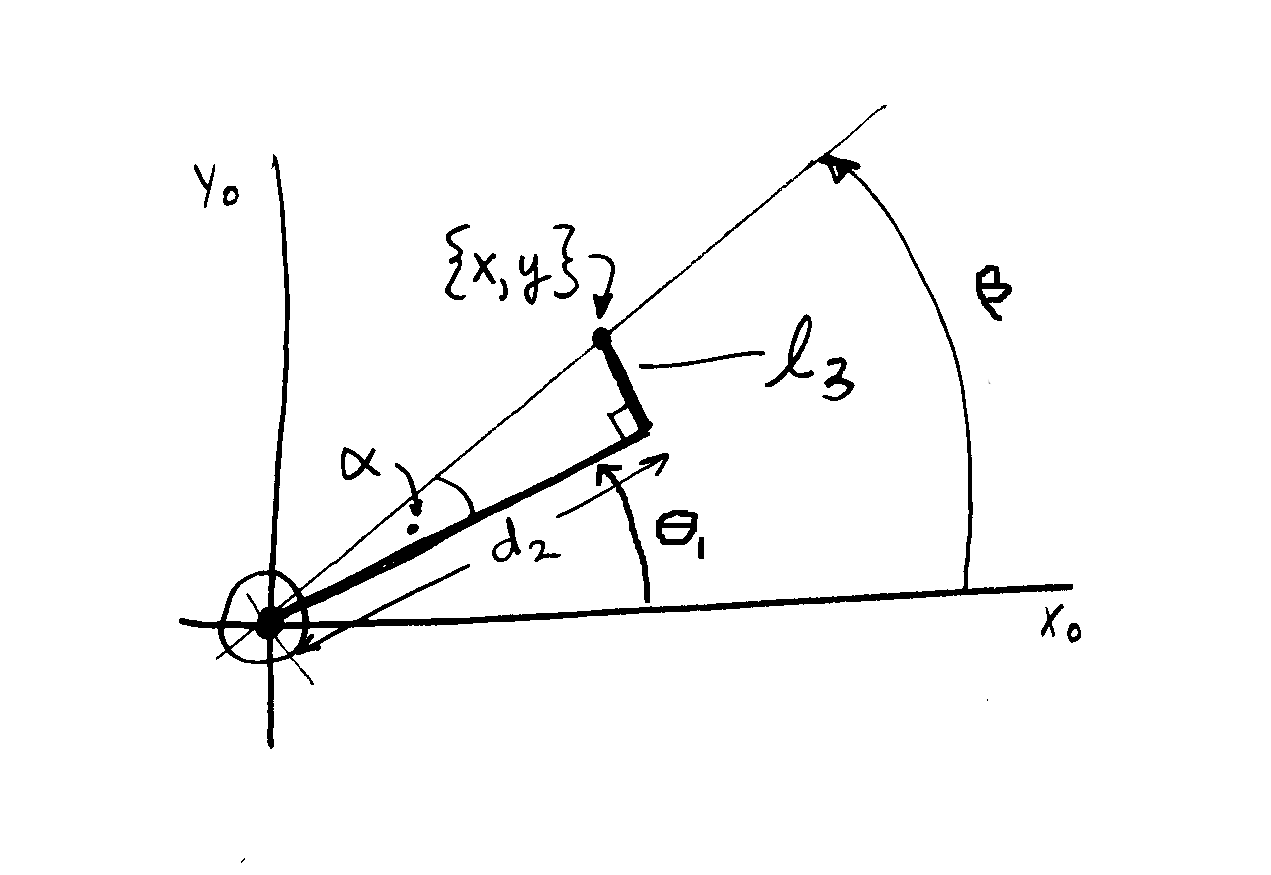
\includegraphics[width=3.5in]{figs04/00088.png}

by Pythagorean theorem and a few basic triangle facts:,
\[
d_2^2 + l_3^2 = x^2 + y^2
\qquad
\beta = \mathrm{atan2}(y,x)
\qquad
\theta_1 = \beta - \alpha
\]
\[
d_2 = \pm\sqrt{x^2 + y^2-l_3^2}
\]
\[
\alpha = \mathrm{atan2}(l_3, d_2)
\]
\[
\theta_1 = \mathrm{atan2}(y,x)-\mathrm{atan2}(l_3, d_2)
\]

There are two solutions, obtained by taking either positive or
negative root of $d_2$.  Choice of $\theta_1$ is automatic.

\end{ExampleSmall}

\begin{Example}

Now assume that $\theta_3$ is variable.
Given $x,y$ and $^0_4R$, or equivalently, the end effector angle, $\gamma$, find $\theta_1, d_2, \theta_3$. How many solutions are there and how do you find them?



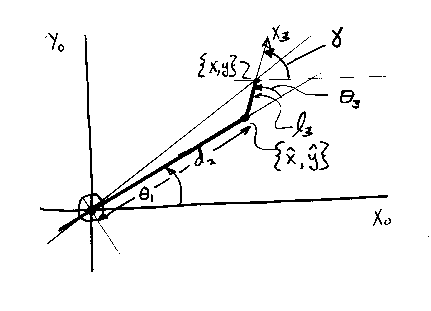
\includegraphics[width=4.5in]{figs04/00089.png}

\subsection*{Solution:}

The manipulator subspace is the set of $T$ matrices which allow a position in the $XY$ plane,
and a rotation angle $\gamma$ of the end effector in the plane:
\[
ManipSS = \begin{bmatrix}
c\gamma & -s\gamma & 0  & x\\
s\gamma & c\gamma & 0  & y\\
0 & 0 &  1 & 0 \\
0&0&0&1
\end{bmatrix}
\]

\[
^0_4R =
\left[ \begin{array}{ccc}
c\gamma & -s\gamma & 0 \\
s\gamma & c\gamma & 0 \\
0 & 0 & 1
\end{array} \right]
\]
\[
\gamma = \mathrm{atan2}(r_{21}, r_{11})
\]
\[
\gamma = \mathrm{direction\, of\,} x_{3}
\]
Now let's solve for the position of the elbow, labeled $\hat{x},\hat{y}$.
\[
\hat{x}=x+l_3\cos(\pi+\gamma)
\]
\[
\hat{y}=y+l_3\sin(\pi+\gamma)
\]
\[
d_2 = \pm \sqrt{\hat{x}^2 + \hat{y}^2}
\]
There are two solutions due to the $\pm$ of the square root.
\[
\theta_{1a}=\mathrm{atan2}(\hat{y},\hat{x})
\]
or
\[
\theta_{1b}=\mathrm{atan2}(\hat{y},\hat{x})+\pi
\]
\[
\theta_{3a} = 90^\circ + \gamma - \theta_1
\]
\[
\theta_{3b} = 90^\circ - \gamma + \theta_1
\]
\end{Example}

\begin{ExampleCont}
There are two solutions, obtained by taking either positive or
negative root of $d_2$.  Add $\pi$ to $\theta_1$ if $d_2 < 0$.
It might be hard to imagine the $d_2<0$ case at first, but look at $x_1$ in the two poses below:
\begin{center}
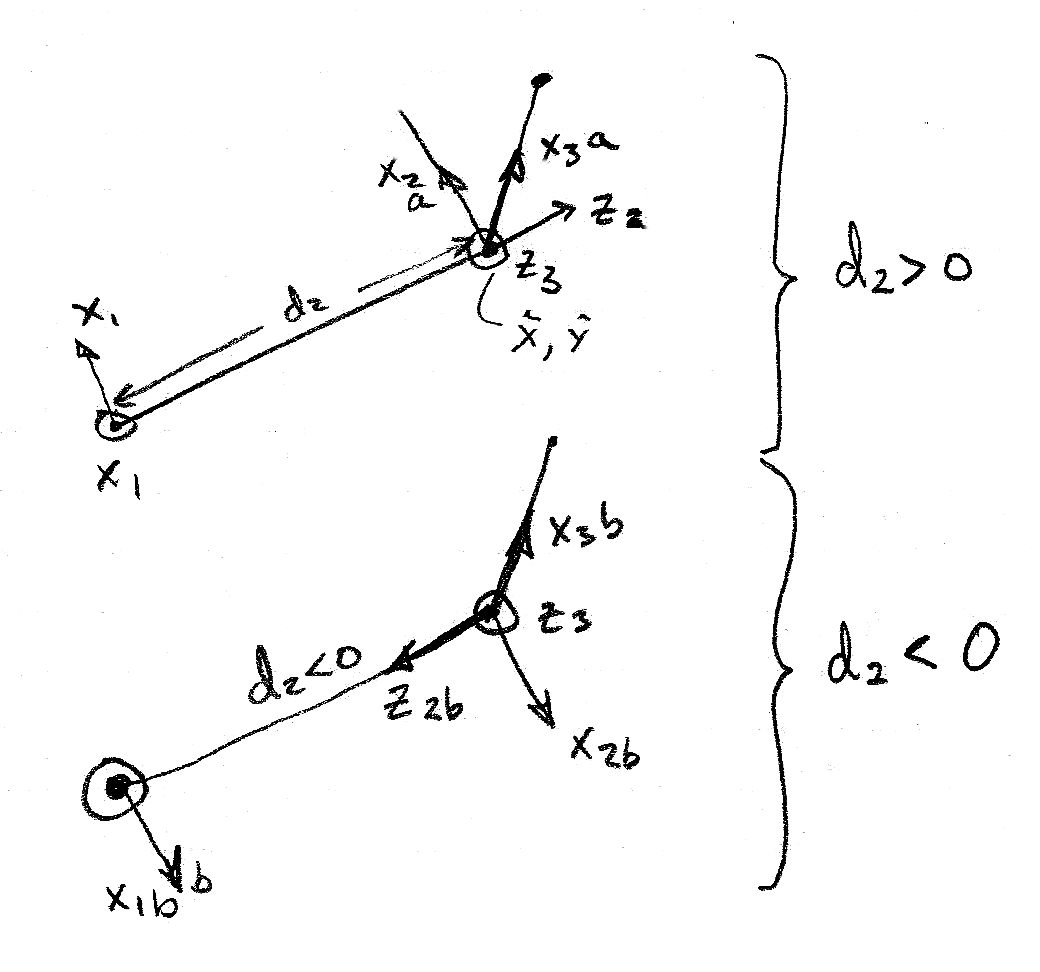
\includegraphics[width=2.5in]{figs04/01125.png}
\end{center}

\end{ExampleCont}


\subsection{Spatial Example}

Now we consider a 3D manipulator in which a plane can be identified (the horizontal plane containing the arm links).

\begin{Example}

\subsection*{SCARA robot arm}

  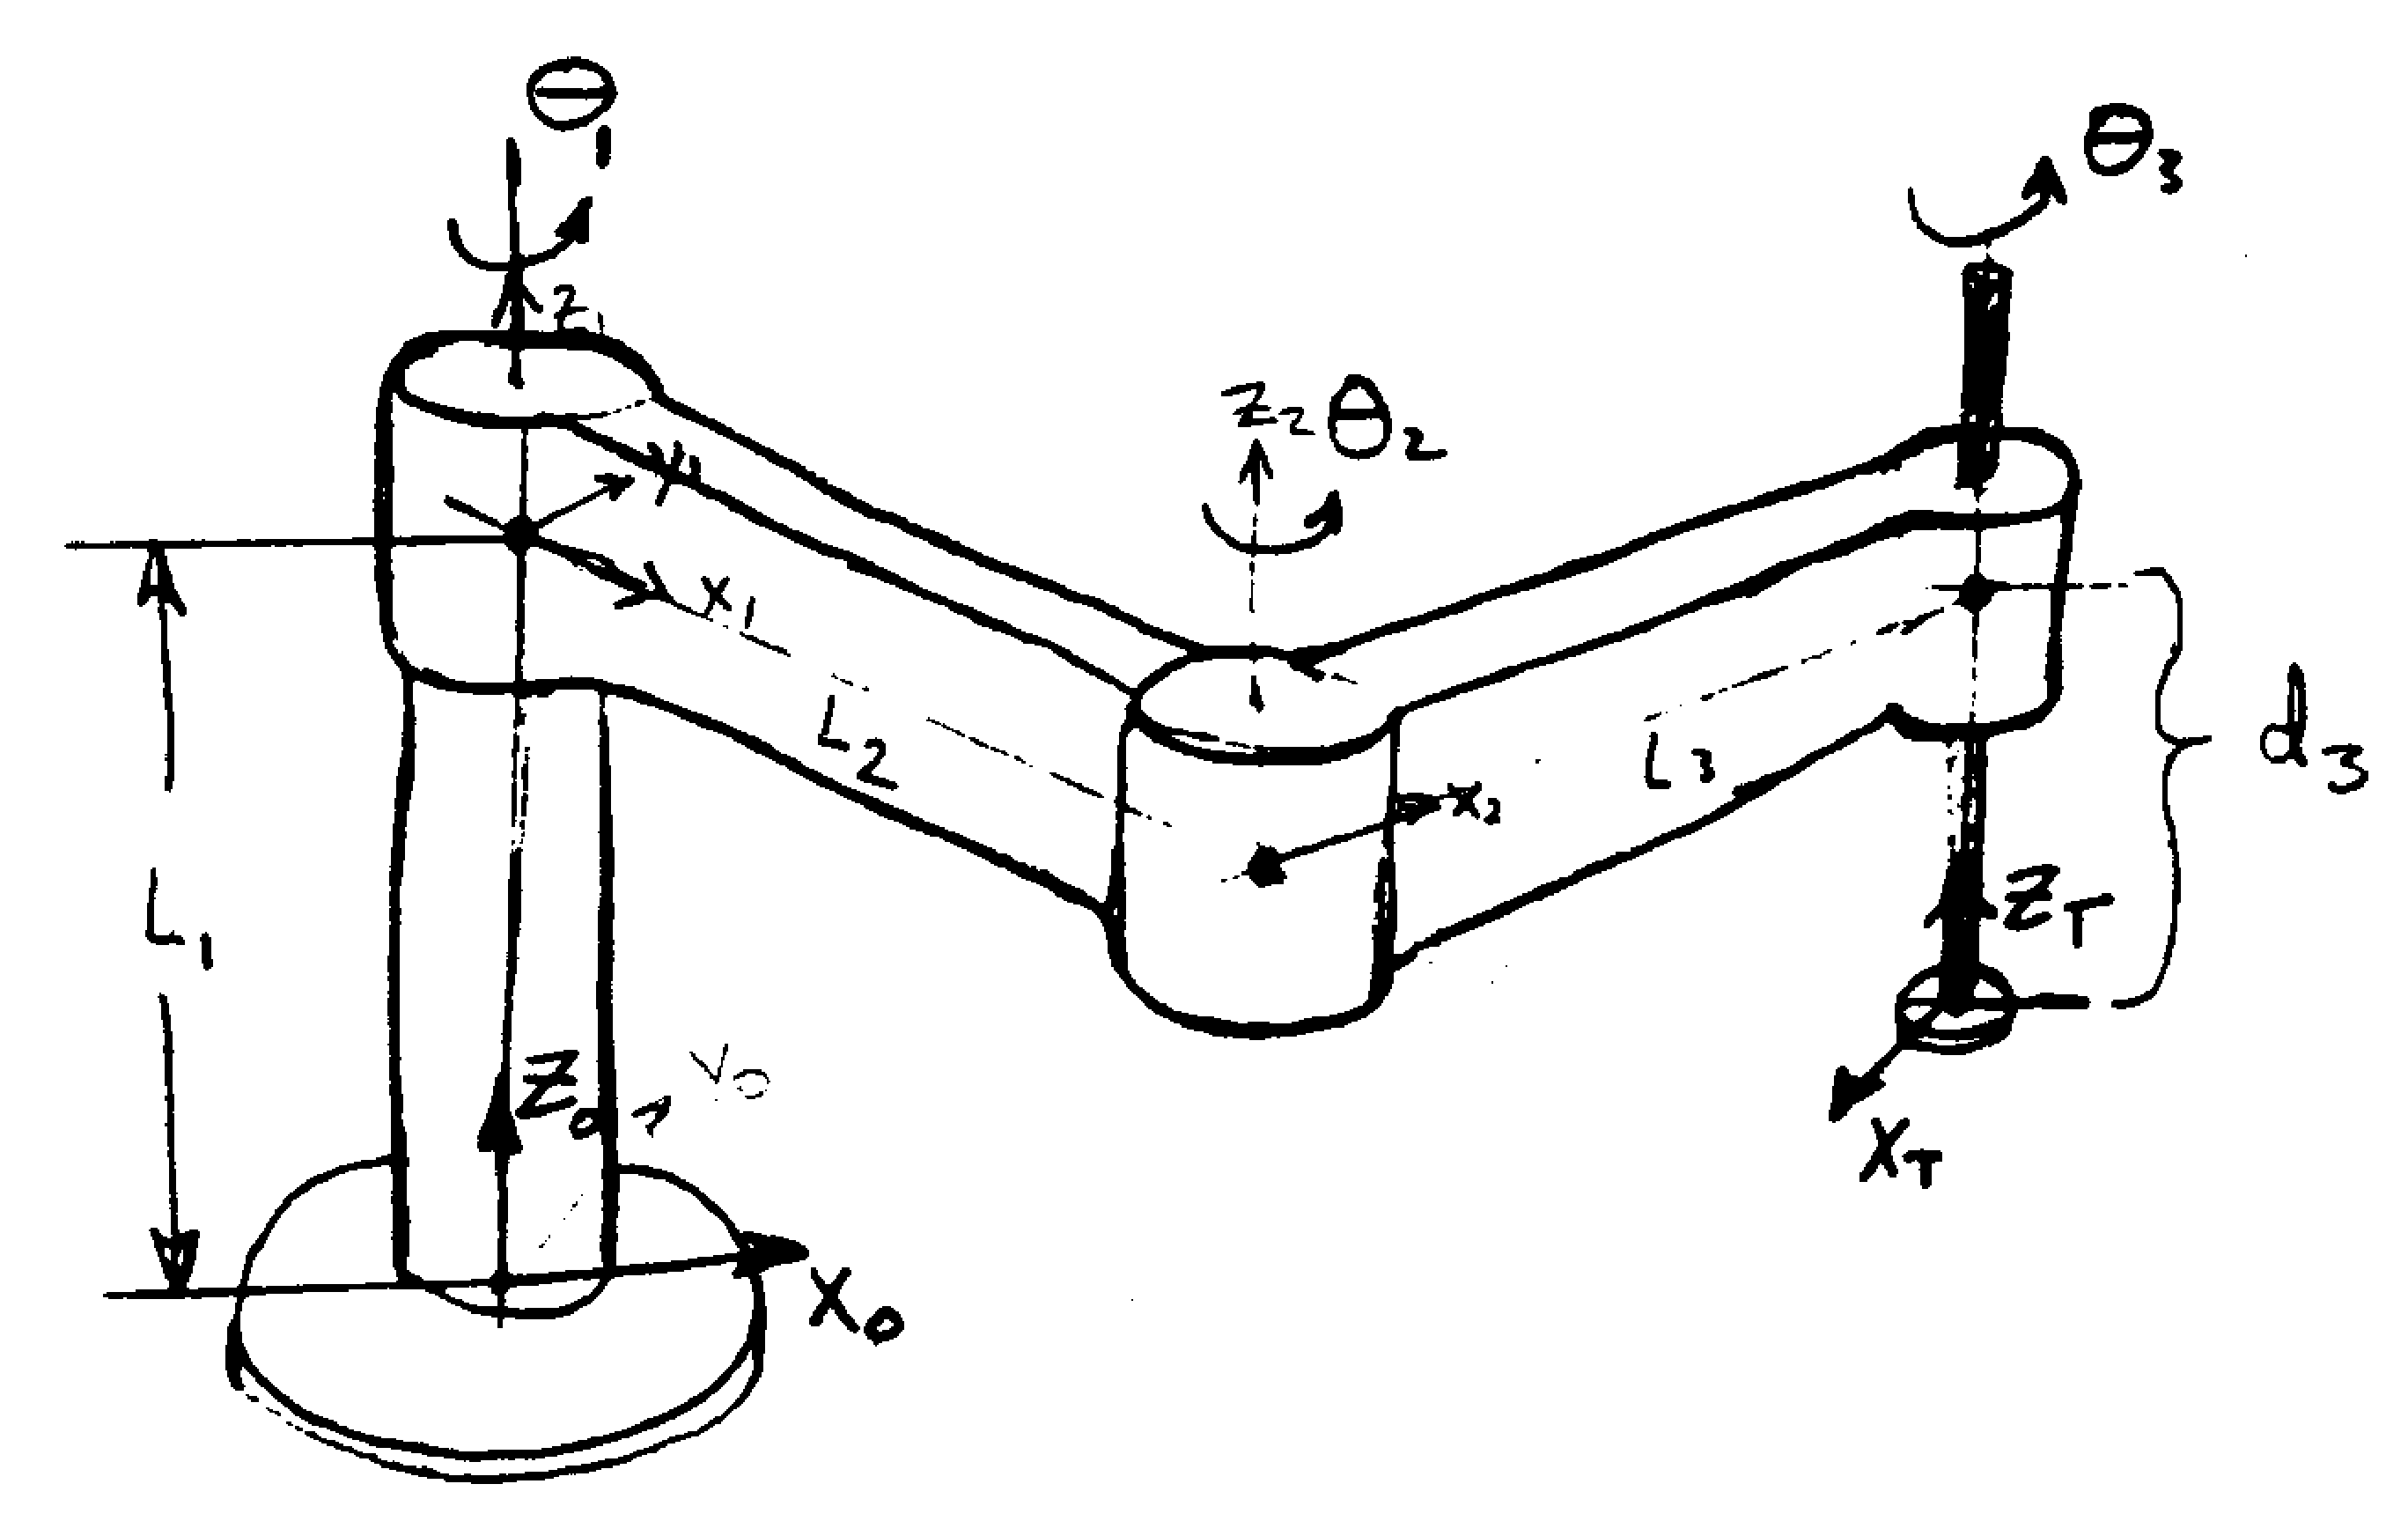
\includegraphics[width=3.5in]{figs04/00253.eps}


This drawing illustrates a type of 4-DOF arm architecture called the  SCARA arm.  All three rotary
axes are parallel and vertical. The manipulator subspace for this robot is
\[
^O_TT_d =
        \left [
        \begin{array}{cccc}
        c\phi   & -s\phi        & 0     &       x_d \\
        s\phi   & c\phi         & 0     & y_d   \\
        0       & 0             & 1     & z_d \\
        0       & 0             & 0     & 1 \\
        \end{array}
        \right ]
\]
where $\phi$ is the rotation of the tool frame in the $X_0, Y_0$ plane. Find the inverse kinematic
solutions for this manipulator, i.e.  find all solutions for $\theta_{1-3}$ and $d_3$ of
\[
^O_TT \left(\left[
        \begin{array}{c}
        \theta_1 \\
        \theta_2 \\
        \theta_3 \\
        d_3\\
        \end{array}
        \right ]
        \right )
   =
^0_TT_d
\]
Since forward kinematic equations are not
given here, the geometric method is preferred.  Make sure you find {\it all} solutions, and
no spurious solutions.

\subsection*{Solution:}

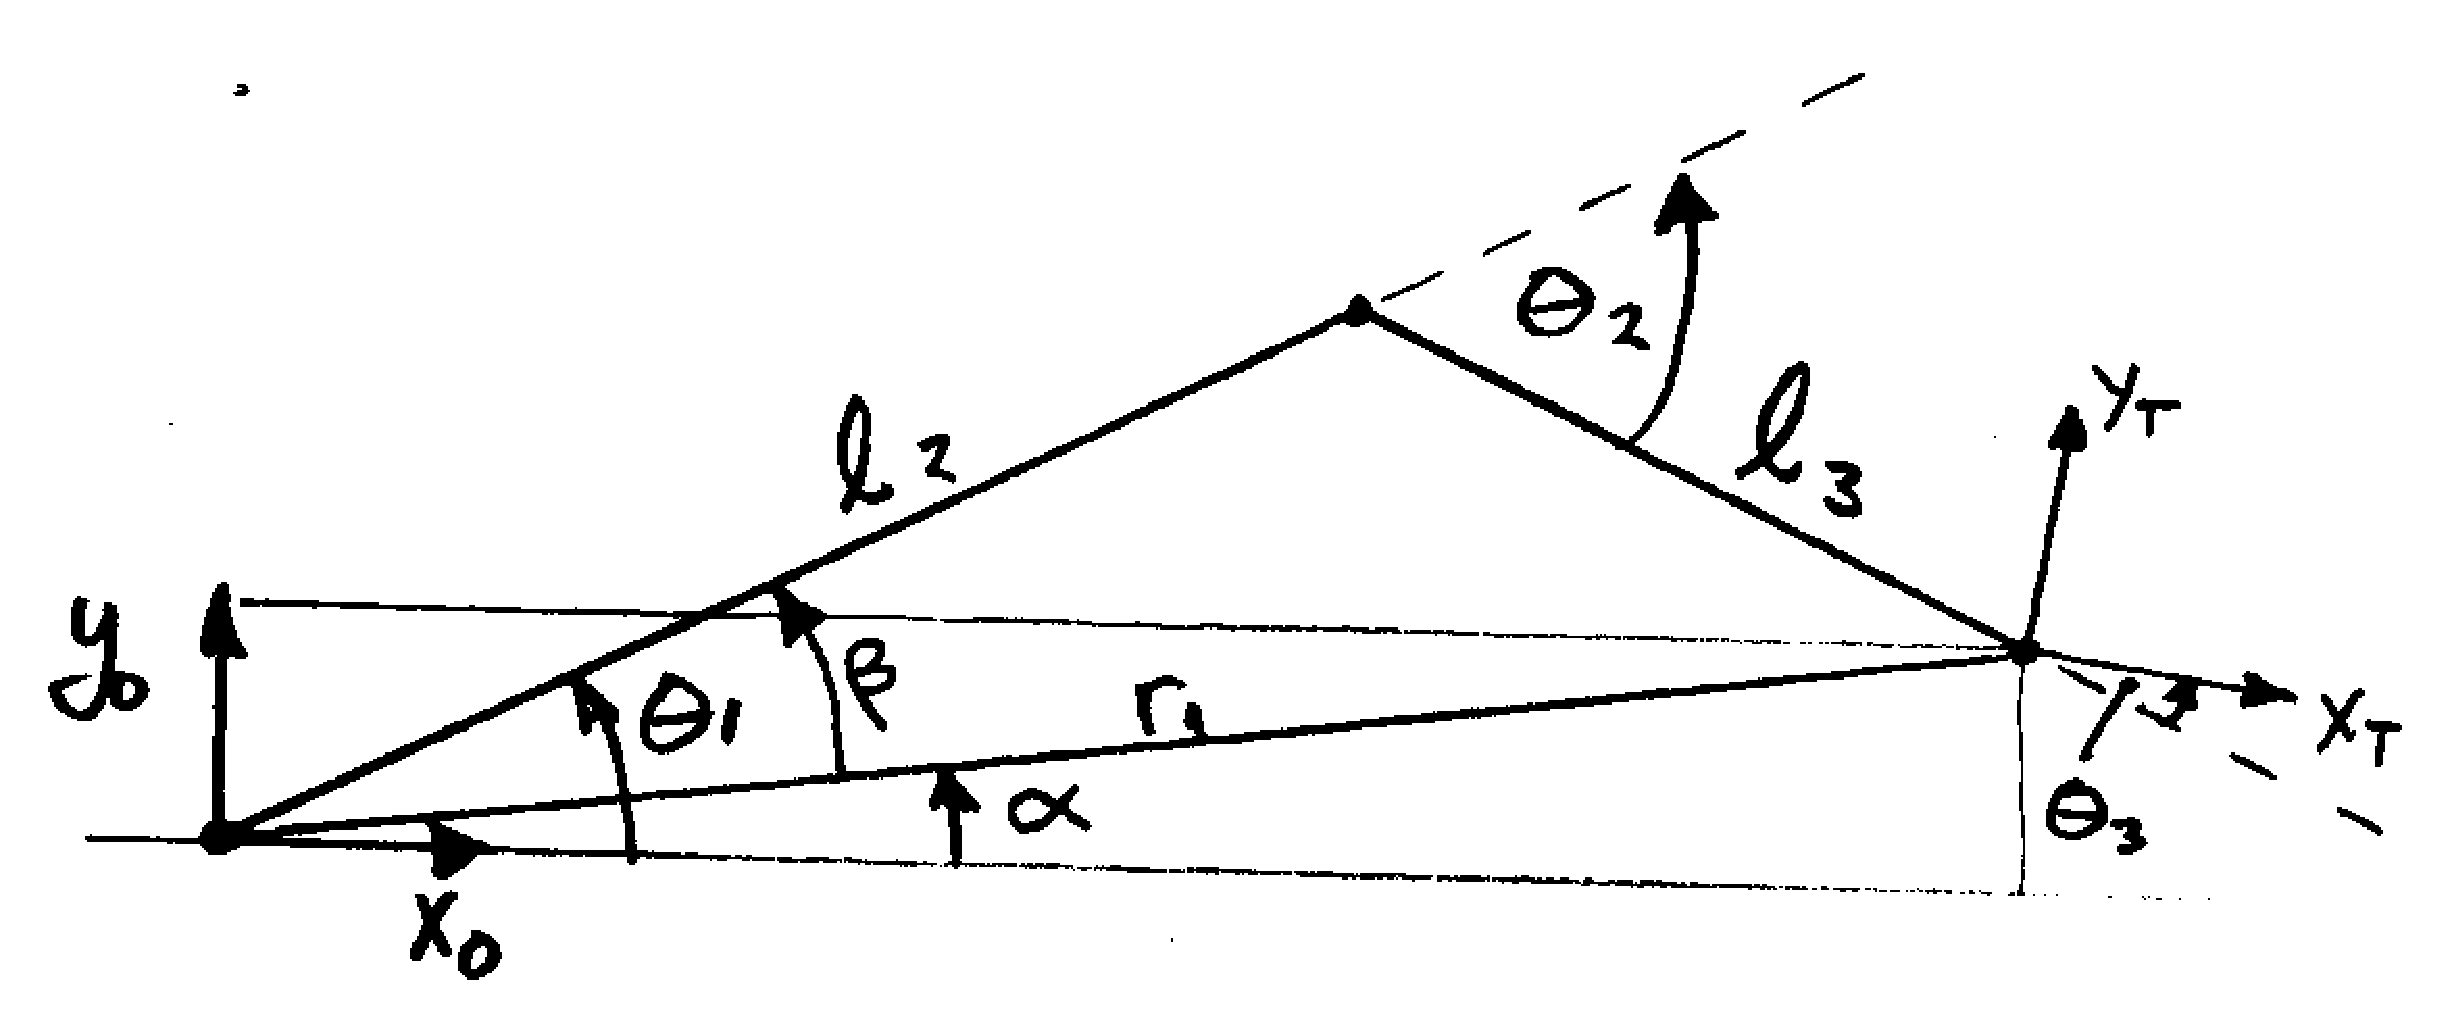
\includegraphics[width=3.5in]{figs04/00254.eps}

The approach is to solve for $\theta_1$ and $\theta_3$ based on the end point $P_0$
and then get $d_3$ and $\theta_3$.

\end{Example}
\newpage
\begin{ExampleCont}
\[
r_1 = +\sqrt{x^2+y^2}
\]
\[
\alpha = \mathrm{atan2}(y_0,x_0)
\]
Using law of cosines,
\[
r_1^2 = l_2^2 + l_3^2 + 2l_2l_3\cos(\theta_2)
\]
\[
\cos(\theta_2) = \frac{r_1^2 - l_2^2 - l_3^2}{2l_2l_3} = r_3
\]
\[
\theta_2 = \pm \cos^{-1}(r_3)
\]
\[
l_3^2 = l_2^2 + r_1^2 - 2l_2r_1\cos\beta
\]
\[
\cos\beta = \frac{l_2^2 + x_0^2+y_0^2-l_3^2}{2l_2r_1} = r_2
\]
\[
\beta = \pm \cos^{-1}(r_2)
\]
\[
\theta_1 = \alpha \pm \beta
\]

\[
\theta_1 = \mathrm{atan2}(y_0,x_0) \pm \cos^{-1}(r_2)
\]
\[
\theta_2 = \pm \cos^{-1}(r_3)
\]
By inspection:
\[
d_3= L1 - z_d
\]
\[
\phi = \mathrm{atan2}(t_{d21}, t_{d11})
\]
where $t_{dij}$ are the elements of $^0_TT_d$. And
\[
\theta_3 = \phi - \theta_1 - \theta_2
\]
\end{ExampleCont}


\section{Summary of Notation}

% Summary of Notation for Chapter  04

